The following chapter describes the specification of the developed system. It is
based on the customer requirements and correspondence with the customer. This
chapter will be adjusted if requirements change, to provide clearance during the
development process, as well as the maintenance process after releasing the
system.

\section{Project Scope}
The system shall support a driver with taking his car out of a parking lot. The
system is designed to work with the cars of the customer. It should use sensors,
build around the car, to take the car out of every parking position in the most
convenient and safe way. The system should provide a graphical user interface
within the car display, to provide overview over the process of taking out the
car.

\section{Supported Parking Positions}
The two main parking positions shall be supported, as shown in the pictures
below:

\begin{figure}[h!]
  \centering
     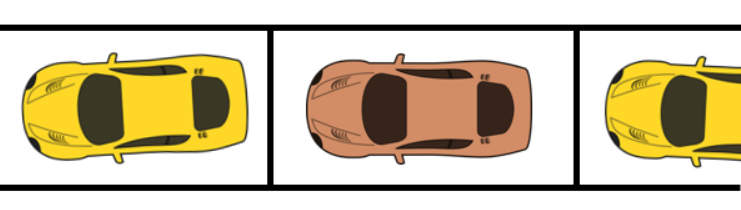
\includegraphics[width=\textwidth]
     {res/spec/Hintereinander.PNG}
     \captionsetup{justification=centering}
  \caption{Parallel Parking}
  \label{fig:project plan}
\end{figure}

\begin{figure}[h!]
  \centering
     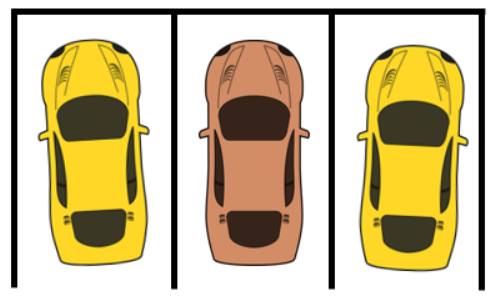
\includegraphics[width=\textwidth]
     {res/spec/Nebeneinander.PNG}
     \captionsetup{justification=centering}
  \caption{Perpendicular Parking}
  \label{fig:project plan}
\end{figure}

\FloatBarrier

A car moved out of a lengthwise parking lot has to face the same direction as
before being taken out, while a car taken out of a transversal parking lot is
moved $90^\circ$ clockwise when being taken out. Angled parking lots are
treated the same way as transversal parking lots, only the orientation of the car is not
changed by the whole $90^\circ$, but by a smaller amount. In all cases, the
cars have to leave the parking lot entirely, and must not enter the opposite lane at any
time of the process.

\section{Sensors}

The system uses a number of sensors placed on and within the automobile. They
are used to ensure a secure process of taking out the vehicle off the parking lot:

\begin{itemize}
 \item	Speed Sensor \newline 
Acquire the current speed 
 \item Distance Sensor \newline
Acquire the distances between the vehicle and obstacles
\end{itemize}

\section{Required Controls}

The parking system requires the control or a possibility to interact with a
number of car components to work properly and to its full potential:

\begin{itemize}
  
\item Transmission control \newline
Switch between forwards and reverse driving
\item Engine control \newline
Set the desired car velocity
\item Board computer control \newline
Display the user interface 
\item Brake control \newline
Decrease the velocity
\item Steering control \newline
Change the vehicles direction
\end{itemize}

The board computer is not mandatory for the system to work, but highly
recommended.

\section{Obstacles}
The parking assistance system shall be able to take obstacles into account.
There are two kinds of obstacles we are facing when running the process of
taking out a car of a parking lot:

\vspace{0.5cm}
\noindent
\textbf{Static obstacles} \newline
Static obstacles are not moving themselves. Their distance towards our vehicle
controlled by the parking assistant system only changes by the movement of the
vehicle itself. We do not have to predict where the obstacle might be positioned
at some other point in time. Static obstacles are objects like:

\begin{itemize}
\item Parked cars
\item Houses 
\item Walls
\item Pavements
\item Trees  
\end{itemize}

\vspace{0.5cm}
\noindent
\textbf{Dynamic obstacles} \newline
Dynamic obstacles have a movement, or the potential to move during our process
of taking out the car of a parking lot. Their distance to our vehicle can change
without our car having any velocity. If there is any possibility, an obstacle
might interfere with our vehicle, or the predicted path of our vehicle, it has
to be taken into account during the process. If the distance between an obstacle
and our vehicle is reducing by a higher ration than the velocity of the car, the
car has to stop. Dynamic obstacles are objects like:

\begin{itemize}
\item Moving cars
\item Human beings
\item Animals  
\end{itemize}

\section{Country Regulations}

The system should primary work in Great Britain � thus the traffic rules of
Britain should be considered when running a process of taking the vehicle out of
the parking lot. The rules for the process do not differ in any country of
Europe by any other factor than the side of the road the cars are driving on.
Therefor there must be a setting to switch between:

\begin{itemize}
 \item Right-hand traffic
 \item Left-hand traffic (default)  
\end{itemize}

\section{Graphical User Interface}

The graphical user interface is a non-mandatory, but highly recommended part of
the system. It shall initiate the process of taking a car out of its parking
position. It shall be intuitive and use the corporate design of the customer.
Furthermore, it shall monitor the process by displaying the following
information to the driver:

\begin{itemize}
 \item	A top-down view of the car and the closest surroundings
 \item Predicted car route
 \item Vehicle velocity
 \item Driving direction
 \item Distance to the closest obstacles on each side of the car
 \item Warnings in case of dangerous situations  
\end{itemize}

\section{Implementation}

The system should be implemented with the programming language C\#. For the
graphical user interface the framework WPF is to be used, as well as the
corporate design of the customer for WPC controls styling. For sensor
communication we will use CAN buses and extract the required information from
the streams. An SQL database will be supplied to assure fast processing of the
high amount of data in a small time and to ensure performance we will work with
stored procedures.
